
\chapter{Experimentos e Resultados}

Este capítulo descreve o desenvolvimento do projeto proposto. O projeto é composto por 5 tarefas de implementação:

\begin{itemize}
    \item Montar os \textit{datasets} de \textit{barcodes} e números;
    \item Treinar, avaliar e selecionar o melhor modelo de rede neural para \textit{barcodes} e números;
    \item Implementar o algoritmo de detecção dos \textit{barcodes}.
    \item Implementar o algoritmo de detecção dos números.
    \item Implementar a aplicação web
\end{itemize}

Utilizaremos a Figura \ref{fig:imagemBase} como referência para a explicação do sistema ao longo do capítulo.

\begin{figure}[h!]
	\centering
	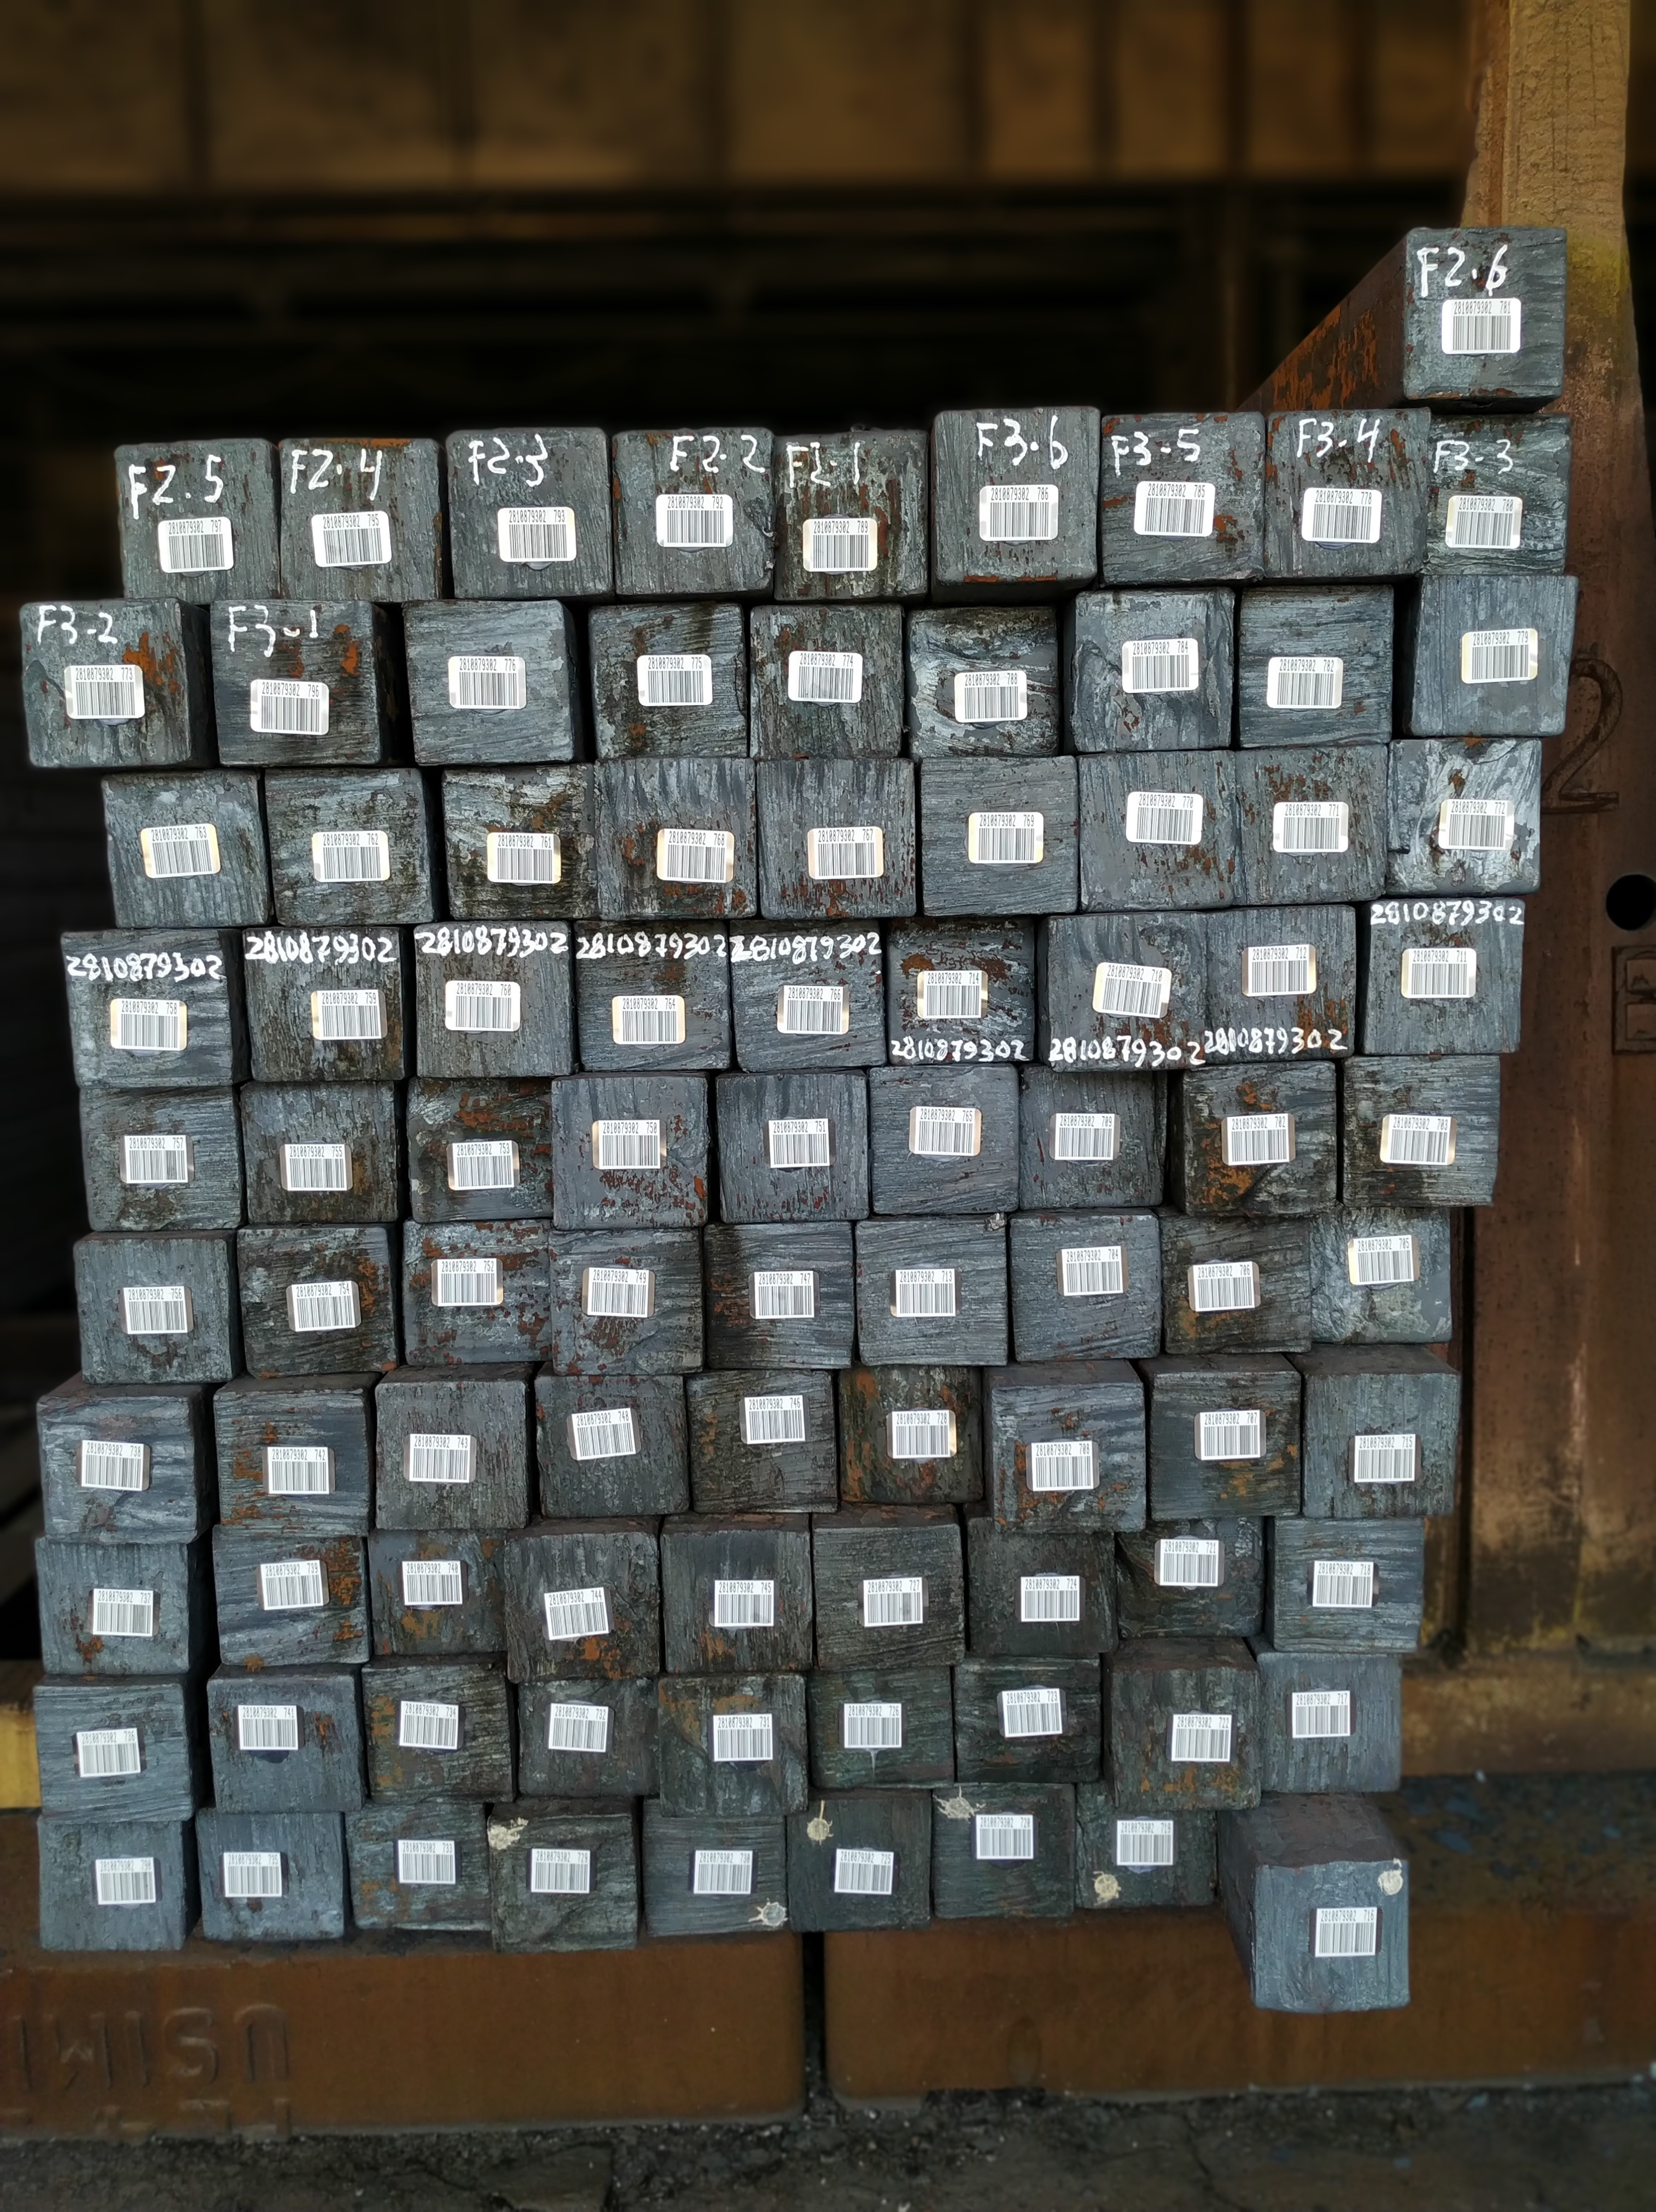
\includegraphics[width=0.5\linewidth]{figuras/img1.jpg}
	\caption{Foto tirada da corrida de tarugos.}
	\label{fig:imagemBase}
\end{figure}

\section{Montagem dos \textit{datasets}}

Nesta seção faremos a montagem dos dois \textit{datasets} para que, posteriormente, as redes neurais sejam treinadas. 

Inicialmente faremos o \textit{download} do conjunto de dados de \textit{barcodes} disponibilizado pelo laboratório \citeauthor{Arte-Lab}. Teremos por volta de 500 imagens de código de barras para o nosso \textit{dataset} inicial.

Criaremos pastas no seguinte modelo de hirarquia para nosso \textit{dataset}. (Código \ref{cod:folders})
\begin{lstlisting}[caption=Hierarquia de pastas para dataset, label=cod:folders][htb!]
        +---barcode
        |   +---train
        |   |   +---annotations
        |   |   \---images
        |   \---validation
        |       +---annotations
        |       \---images
        
        +---number
        |   +---train
        |   |   +---annotations
        |   |   \---images
        |   \---validation
        |       +---annotations
        |       \---images
\end{lstlisting}

Através do método \textit{Data Augmentation} \ref{sec:dataAugm}, aumentaremos nossa base de dados para que, após o treino, a acurácia do modelo de nossa rede neural seja a maior possível. Aplicaremos o modelo nas imagens 500 imagens resultando em $\sim~1500$ imagens de código de barras.

Utilizando a Figura \ref{fig:imagemBase}, cortaremos as etiquetas com a ajuda do software \textit{Paint} do \textit{Windows}, para sera gerada nossa base de dados de números. Optamos por utilizar os números localizados nas etiquetas uma vez que foram feitos diversos treinamento com fontes numéricas diferentes e, portanto, não obtivemos uma acurácia de detecção do número esperada.(Figura \ref{fig:barcodeDataset})

\begin{figure}[htbp]
	\centering
	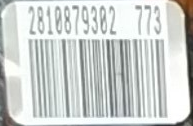
\includegraphics[width=0.25\linewidth]{figuras/MachineLearning/barcodeDataset.png}
	\caption{Montagem \textit{dataset} de números}
	\label{fig:barcodeDataset}
\end{figure}

Colocaremos 75\% das imagens na pasta validation e resto em train tanto no \textit{dataset} de \textit{barcodes} como no de números.

\subsection{Anotações das imagens}

Utilizando o software LabelImg (Subseção \ref{sub:LabelImg}), faremos as anotações das imagens para que seja gerado o arquivo PASCAL VOC no formato XML. (Figura \ref{fig:barNumAn})

\begin{figure}[htbp]
	\centering
	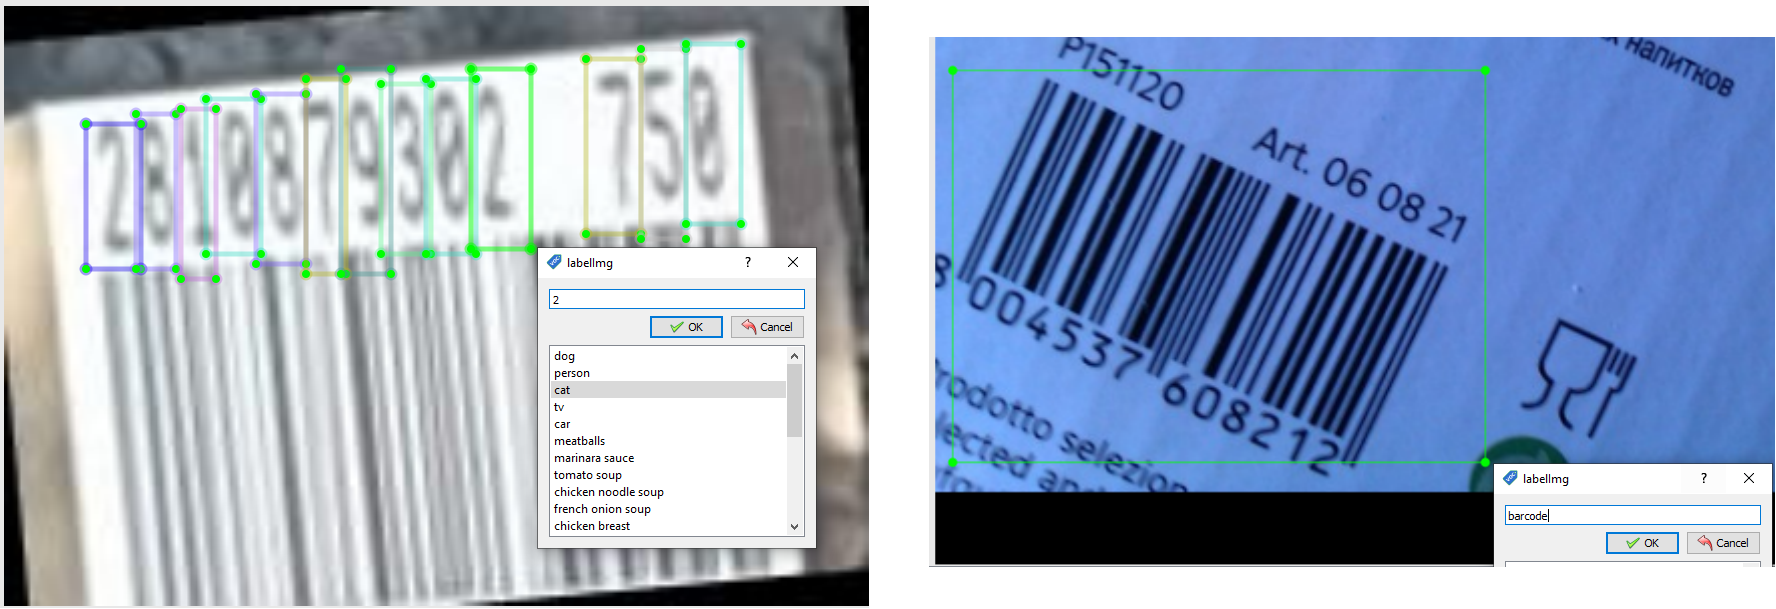
\includegraphics[width=1\linewidth]{figuras/MachineLearning/barNumAn.png}
	\caption{Anotações das imagens (Números e \textit{Barcodes})}
	\label{fig:barNumAn}
\end{figure}

\section{Fase de treinamento}

Nesta seção iremos treinar, avaliar e selecionar o melhor modelo de \textit{barcode} e número a partir da rede neural pré-treinada YOLOv3 (Subseção \ref{sub:Yolov3}).

\subsection{Treinando o modelo}

Utilizando a biblioteca ImageAI, e importando a classe \textit{DetectionModelTrainer}, treinaremos o modelo (Código \ref{cod:modeTrain}).

\begin{lstlisting}[caption=Exemplo de código do método \textit{data augmentation}, label=cod:modeTrain][htb!]
from imageai.Detection.Custom import DetectionModelTrainer

trainer = DetectionModelTrainer()
trainer.setModelTypeAsYOLOv3()
trainer.setDataDirectory(data_directory="barcode")
trainer.setTrainConfig(object_names_array=["barcode"], batch_size=4, 
                        num_experiments=11, 
                        train_from_pretrained_model=
                                            "pretrained-yolov3.h5")
trainer.trainModel()
\end{lstlisting}

\begin{itemize}
    \item \textit{object\_names\_array}: matriz que contém os nomes dos objetos em nosso \textit{dataset};
    \item \textit{batch\_size}: indica o tamanho do \textit{batch} para o treinamento;
    \item \textit{num\_experiments}: indica o número de vezes que a rede treinará sobre todas as imagens de treinamento, também chamadas de \textit{Epochs};
\end{itemize}

\begin{figure}[htbp]
	\centering
	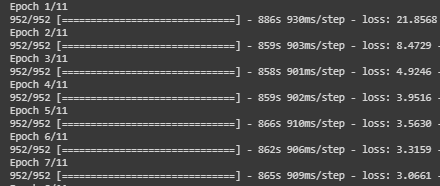
\includegraphics[width=1\linewidth]{figuras/MachineLearning/barcodeTraining.png}
	\caption{Anotações das imagens (Números e \textit{Barcodes})}
	\label{fig:barTrain}
\end{figure}

    A figura acima significa o progresso do treinamento.
\begin{itemize}
    \item Para cada experimento (\textit{Epoch}), a perda total geral de validação (por exemplo - \textit{loss}: 4.7582) é relatada.
    \item Para cada queda em \textit{loss} após uma experiência, um modelo é salvo na pasta barcode/models. Quanto menor a perda, melhor o modelo, de um modo geral, é desenhada para mostrar o quão longe estamos da solução "ideal". 
\end{itemize}

O método \textit{trainer.evaluateModel} mostrará as métricas de saída de cada modelo e a partir dos modelos gerados, avaliaremos o mAP \footnote{AP (precisão média) é uma métrica popular na medição da precisão de detectores de objetos;} de cada modelo de detecção salvo.  (Código \ref{cod:metrics})

\begin{lstlisting}[caption=Métricas de saída do modelo, label=cod:metrics][htb!]
metrics = trainer.evaluateModel(model_path="detection_model-ex-013--loss-0003.066.h5", json_path="detection_config_barcode.json", iou_threshold=0.5, object_threshold=0.3, nms_threshold=0.5)
\end{lstlisting}

Obtivemos o seguintes resultados para nossos modelos de barcodes e números:

\begin{table}[H]
	\centering
	\begin{tabular}{|l|l|l|}
		\hline
		\rowcolor[HTML]{ECF4FF} 
		\multicolumn{1}{|c|}{\cellcolor[HTML]{ECF4FF}\textit{Característica}} &
		\multicolumn{1}{|c|}{\cellcolor[HTML]{ECF4FF}\textit{Barcode}} & \multicolumn{1}{c|}{\cellcolor[HTML]{ECF4FF}\textit{Number}}\\ \hline
		\textit{Epochs} & 7 & 53\\ \hline
		\textit{Loss} & 3.066 & 12.296\\ \hline
		\textit{mAP} & 91.07\% & 77.90\%  \\ \hline
	\end{tabular}
	\caption{Melhores resultados encontrados nos modelos.}
	\label{tab:Result}
\end{table}

Ao detalhar a média de precisão dos números, podemos observar a porcentagem da probabilidade de cada número.

\begin{table}[H]
	\centering
	\begin{tabular}{|l|l|l|}
		\hline
		\rowcolor[HTML]{ECF4FF} 
		\multicolumn{1}{|c|}{\cellcolor[HTML]{ECF4FF}\textit{\textit{Number}}} &
		\multicolumn{1}{|c|}{\cellcolor[HTML]{ECF4FF}\textit{Média}}\\ \hline 
		0&  78.38\% \\ \hline
		1&  49.64\% \\ \hline
		2&  85.21\% \\ \hline
		3&  78.55\%\\ \hline
		4&  83.47\% \\ \hline
		5&  67.46\% \\ \hline
		6&  80.00\% \\ \hline
		7&  85.66\% \\ \hline
		8&  84.31\% \\ \hline
		9&  86.36\% \\ \hline
		mAP&  77.90\% \\ \hline 
		
	\end{tabular}
	\caption{Médias de precisões dos números.}
	\label{tab:avgNumbersResult}
\end{table}


\section{Implementação dos algoritmos de detecção}

Nesta seção iremos implementar os algoritmos de detecção de \textit{barcodes} e números utilizando os modelos de redes reunais treinadas na seção anterior.

\subsection{Detecção de \textit{barcode}}

Para 

\subsection{Detecção de número}


\section{Aplicação Web}